El fin de trabajar con dos modelos, el de regresión lineal y la red neuronal, es para comparar su desempeño y así mismo, sus respectivos resultados. Cabe destacar que el año ``objetivo'' es el 2040.

\subsubsection{Modelo de Regresión Lineal}

De manera concisa, el número total de muertes estimadas para el año 2040 por el Modelo de Regresión Lineal son: \textbf{10461.07}, proporcionándonos el siguiente gráfico: 

\begin{figure}[H] \centering 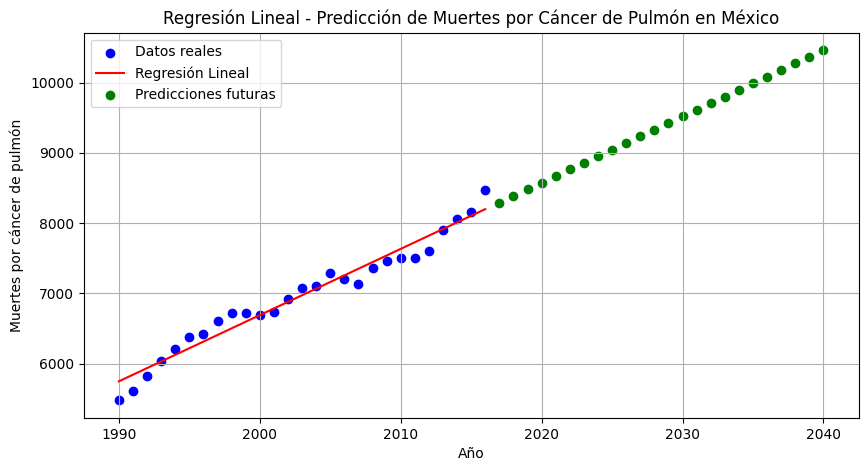
\includegraphics[width=0.70\textwidth]{Zdenko/Imágenes/regresion.png} \caption{Modelo de Regresión Lineal} \label{fig:regresion} \end{figure}

Como se puede apreciar, la evolución es completamente lineal.

\subsubsection{Red Neuronal Recurrente (LTSM)}

Por parte de la red neuronal concurrente, su predicción es de \textbf{7815.07}, arrojándonos el siguiente gráfico: 

\begin{figure}[h] \centering 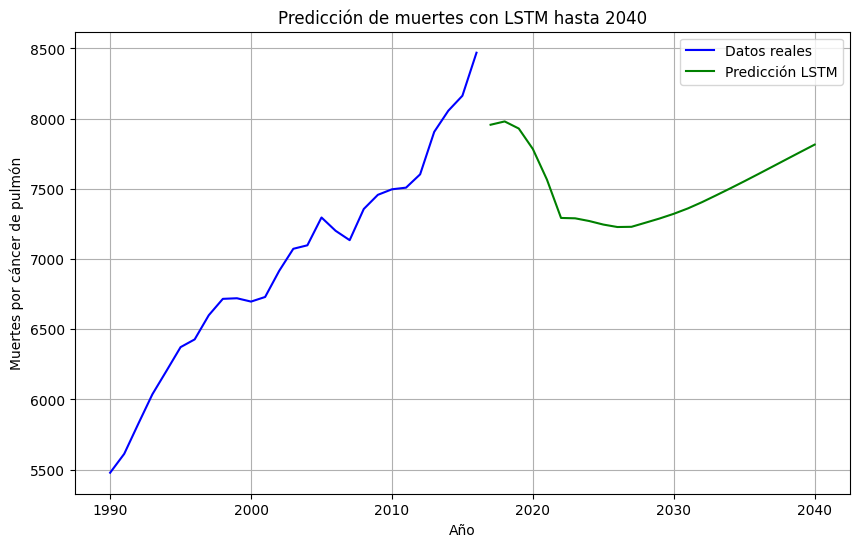
\includegraphics[width=0.85\textwidth]{Zdenko/Imágenes/red.png} \caption{Modelo LSTM} \label{fig:red} \end{figure}

A diferencia del modelo de regresión lineal, la red neuronal LSTM muestra un comportamiento menos lineal, adaptándose al conjunto de datos estudiados. 

\subsubsection{Comparación entre modelos}

Existe cierta cantidad de cálculo para la comparación entre diversos modelos, tales son: Error Absoluto Medio (MAE, por sus siglas en inglés), Error Cuadrático Medio (MSE, por sus siglas en inglés), Coeficiente de Determinación (R²); no obstante, en esta ocasión, solo nos centraremos en el MSE para realizar la comparación de desempeño y resultados entre ambos modelos.

\begin{figure}[H] 
    \centering 
    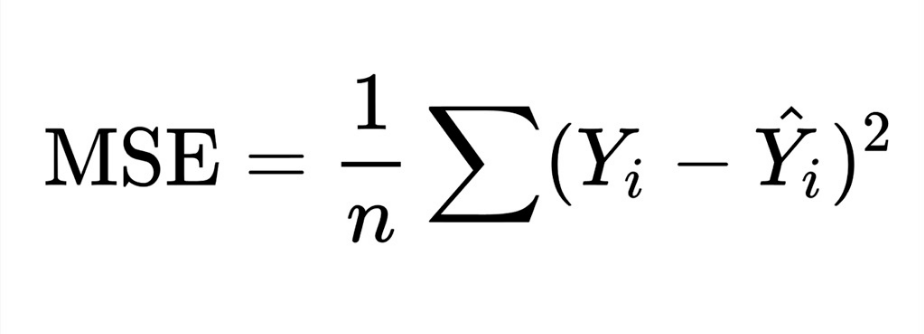
\includegraphics[width=0.5\textwidth]{Zdenko/Imágenes/formula_MSE.png} 
    \caption{Fórmula MSE} 
    \label{fig:formula} 
\end{figure}


El porqué radica en que en general, un MSE más bajo indica que el modelo está haciendo predicciones más precisas, ya que el error cuadrático castiga los errores grandes, lo que impulsa a los modelos a evitar grandes desviaciones. Es particularmente útil cuando deseas evitar errores muy grandes en las predicciones, como es el caso con las muertes causadas por cáncer de pulmón, donde un error grande podría tener consecuencias graves.

En este momento, estamos enfocados en observar qué modelo cuenta con un MSE menor. 

El cálculo del MSE tanto en el modelo de regresión lineal y la red neuronal LSTM fue realizado con la librería sklearn.metrics, haciendo uso de su método: "mean squared error".

\lstset{
    language=Python, % Define el lenguaje
    basicstyle=\ttfamily, % Configura la fuente del texto
    keywordstyle=\color{blue}, % Resalta las palabras clave en azul
    commentstyle=\color{green}, % Comentarios en verde
    stringstyle=\color{red}, % Cadenas de texto en rojo
    breaklines=true, % Permite saltos de línea en el código
}

\begin{lstlisting}
mse = mean_squared_error(y_test, y_pred)
\end{lstlisting}

\newpage

Por parte de la red neuronal, primero se desnormalizaron las predicciones para estar dentro del mismo rango de valores y posterior a eso, se aplicó el método de la librería: 

\lstset{
    language=Python,
    basicstyle=\ttfamily\footnotesize,
    keywordstyle=\color{blue},
    commentstyle=\color{gray},
    stringstyle=\color{green!60!black},
    numberstyle=\tiny\color{gray},
    numbers=left,
    breaklines=true,
    frame=single,
    captionpos=b,
    tabsize=4,
    showspaces=false,
    showstringspaces=false,
    showtabs=false
}

\begin{lstlisting}
# Hacer predicciones con el modelo LSTM en el conjunto de prueba
y_pred_lstm = model.predict(X_test)

# Desnormalizar las predicciones de la LSTM
y_pred_lstm_original = scaler_y.inverse_transform(y_pred_lstm)
y_test_original = scaler_y.inverse_transform(y_test)

# Calcular MSE con valores originales
mse_lstm = mean_squared_error(y_test_original, y_pred_lstm_original)
\end{lstlisting}

Dichos cálculos fueron útiles para realizar un gráfico y comparar sus resultados.
\begin{figure}[H] \centering 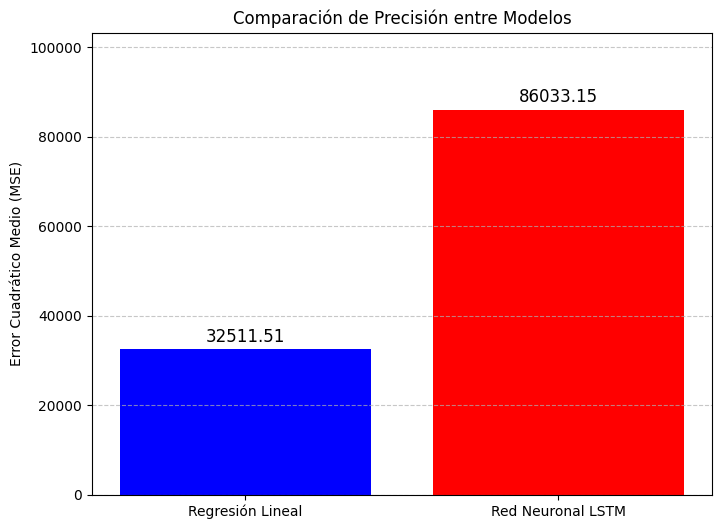
\includegraphics[width=0.75\textwidth]{Zdenko/Imágenes/comparacion.png} \caption{MSE en ambos modelos} \label{fig:comparacion} \end{figure}

Señalando que el modelo de regresión lineal, es más apropiado para este caso. 